\documentclass{article}

\usepackage[utf8]{inputenc}
\usepackage[margin=1in]{geometry}
\usepackage{amsmath, amssymb, amsthm}
% enumitem not available in this TeX installation
\usepackage{hyperref}
\usepackage{booktabs}
\usepackage{tikz}
\usetikzlibrary{arrows.meta, positioning, calc, shapes.geometric}

% --- Theorem environments ---
\newtheorem{theorem}{Theorem}[section]
\newtheorem{lemma}[theorem]{Lemma}
\newtheorem{corollary}[theorem]{Corollary}
\newtheorem{definition}[theorem]{Definition}
\newtheorem{proposition}[theorem]{Proposition}
\newtheorem{example}{Example}[section]

\theoremstyle{remark}
\newtheorem*{remark}{Remark}

% --- Indent subsection headings and content ---
\newlength{\subsecindent}
\setlength{\subsecindent}{2em}

\makeatletter
\renewcommand\subsection{\@startsection{subsection}{2}{\subsecindent}%
  {-3.25ex\@plus -1ex \@minus -.2ex}%
  {1.5ex \@plus .2ex}%
  {\normalfont\large\bfseries}}
\makeatother

\newenvironment{sub}{%
  \begin{list}{}{%
    \setlength{\leftmargin}{4em}%
    \setlength{\rightmargin}{0pt}%
    \setlength{\topsep}{0pt}%
    \setlength{\partopsep}{0pt}%
    \setlength{\parsep}{\parskip}%
    \setlength{\itemsep}{\parskip}%
  }\item\relax
}{\end{list}}

\newenvironment{secbody}{%
  \begin{list}{}{%
    \setlength{\leftmargin}{\subsecindent}%
    \setlength{\rightmargin}{0pt}%
    \setlength{\topsep}{0pt}%
    \setlength{\partopsep}{0pt}%
    \setlength{\parsep}{\parskip}%
    \setlength{\itemsep}{\parskip}%
  }\item\relax
}{\end{list}}

% --- Custom commands ---
\newcommand{\E}{\mathbb{E}}
\newcommand{\Var}{\operatorname{Var}}
\newcommand{\SD}{\operatorname{SD}}
\newcommand{\Prob}{\mathbb{P}}
\newcommand{\given}{\mid}
\newcommand{\R}{\mathbb{R}}

\title{Chapter 2: Discrete Random Variables and Probability Distributions}
\author{MATH 33305 --- Study Notes}
\date{\today}

\begin{document}
\maketitle
\tableofcontents
\newpage

%%%%%%%%%%%%%%%%%%%%%%%%%%%%%%%%%%%%%%%%%%%%%%%%%%%%%%%%%%%%%
%%%%%%%%%%%%%%%%%%%%%%%%%%%%%%%%%%%%%%%%%%%%%%%%%%%%%%%%%%%%%
\part{Outline}
\label{part:outline}
%%%%%%%%%%%%%%%%%%%%%%%%%%%%%%%%%%%%%%%%%%%%%%%%%%%%%%%%%%%%%
%%%%%%%%%%%%%%%%%%%%%%%%%%%%%%%%%%%%%%%%%%%%%%%%%%%%%%%%%%%%%

% ==========================================================
\section{Discrete Random Variables (Sections 2.1--2.2)}
% ==========================================================

\begin{secbody}
\begin{itemize}
  \item[\textbf{A.}] \textbf{Random Variable} --- A function $X: S \to \R$ mapping outcomes to real numbers.
  \item[\textbf{B.}] \textbf{Discrete Random Variable} --- Possible values are finite or countably infinite.
  \item[\textbf{C.}] \textbf{Probability Mass Function (PMF)} --- $f(x) = P(X = x)$; properties: non-negativity, total probability.
  \item[\textbf{D.}] \textbf{Cumulative Distribution Function (CDF)} --- $F(x) = P(X \le x)$; step function, right-continuous, non-decreasing.
\end{itemize}
\end{secbody}

% ==========================================================
\section{Expected Value, Variance, and Standard Deviation (Section 2.3)}
% ==========================================================

\begin{secbody}
\begin{itemize}
  \item[\textbf{E.}] \textbf{Expected Value} --- $\mu = \E(X) = \sum_{\text{all } x} x\, f(x)$; long-run average.
  \item[\textbf{F.}] \textbf{Expected Value of a Function} --- $\E(u(X)) = \sum u(x) f(x)$; linearity of $\E$.
  \item[\textbf{G.}] \textbf{Variance} --- $\sigma^2 = \E(X^2) - \mu^2$; measures spread.
  \item[\textbf{H.}] \textbf{Standard Deviation} --- $\sigma = \sqrt{\sigma^2}$; same unit as $X$.
  \item[\textbf{I.}] \textbf{Mean and Variance of $a + bX$} --- $\E(a+bX) = a + b\mu$, $\Var(a+bX) = b^2 \sigma^2$.
\end{itemize}
\end{secbody}

% ==========================================================
\section{Common Discrete Distributions}
% ==========================================================

\begin{secbody}
\begin{itemize}
  \item[\textbf{A.}] \textbf{Discrete Uniform} (Section 2.1) --- $f(x) = 1/k$, $x = 1, \ldots, k$.
  \item[\textbf{B.}] \textbf{Hypergeometric} (Section 2.10) --- Sampling without replacement from two types.
  \item[\textbf{C.}] \textbf{Binomial} (Section 2.4) --- $n$ independent Bernoulli trials; includes Bernoulli as $n=1$ case.
  \item[\textbf{D.}] \textbf{Moment Generating Function (MGF)} --- $M_X(t) = \E(e^{tX})$; moments, skewness, kurtosis.
  \item[\textbf{E.}] \textbf{Geometric \& Negative Binomial} (Section 2.9) --- Trials until $r$-th success.
  \item[\textbf{F.}] \textbf{Poisson} (Section 2.14) --- Count of events in an interval; limit of Binomial.
\end{itemize}
\end{secbody}

% ==========================================================
\section{Key Relationships}
% ==========================================================

\begin{secbody}
\begin{itemize}
  \item $\text{Bin}(1,p) \equiv \text{Ber}(p)$
  \item $\text{Geometric}(p) \equiv \text{NB}(1,p)$
  \item $\text{HG}(N, N_1, n) \approx \text{Bin}(n, N_1/N)$ when $n/N \le 0.05$
  \item $\text{Bin}(n,p) \approx \text{Poisson}(np)$ when $n$ is large and $p$ is small
  \item Poisson is the limiting distribution of Binomial
\end{itemize}
\end{secbody}


%%%%%%%%%%%%%%%%%%%%%%%%%%%%%%%%%%%%%%%%%%%%%%%%%%%%%%%%%%%%%
%%%%%%%%%%%%%%%%%%%%%%%%%%%%%%%%%%%%%%%%%%%%%%%%%%%%%%%%%%%%%
\newpage
\part{Overview --- First Pass through Chapter 2}
\label{part:overview}
%%%%%%%%%%%%%%%%%%%%%%%%%%%%%%%%%%%%%%%%%%%%%%%%%%%%%%%%%%%%%
%%%%%%%%%%%%%%%%%%%%%%%%%%%%%%%%%%%%%%%%%%%%%%%%%%%%%%%%%%%%%

% ==========================================================
\section{Random Variables and Their Descriptions}
\label{sec:ov-rv}
% ==========================================================

\subsection{Random Variable}
\begin{sub}

A \textbf{random variable} $X$ is a function that assigns a real number to each outcome $w$ in the sample space $S$:
\[
  X_{(w)} = x, \quad w \in S, \; x \in \R.
\]
A random variable is \textbf{discrete} if its set of possible values is finite or countably infinite.

\end{sub}

\subsection{Probability Mass Function (PMF)}
\begin{sub}

The PMF of a discrete r.v.\ $X$ is defined as
\[
  \boxed{f(x) = P(X = x), \quad \text{for all } x \text{ such that } f(x) > 0.}
\]

\textbf{Properties:}
\begin{enumerate}
  \item $0 \le f(x) \le 1$ for any $x$.
  \item $\displaystyle\sum_{\text{all } x} f(x) = 1$. \quad (Total probability)
  \item $\displaystyle P(a < X \le b) = \sum_{a < x \le b} f(x)$. \quad (Sum the PMF)
\end{enumerate}

A PMF can be represented by: a table, a formula, or a graph.

\end{sub}

\subsection{Cumulative Distribution Function (CDF)}
\begin{sub}

The CDF of r.v.\ $X$ is
\[
  \boxed{F(x) = P(X \le x) = \sum_{k \le x} P(X = k), \quad x \in \R.}
\]

\textbf{Key properties of $F(x)$} when $X$ is discrete:
\begin{itemize}
  \item Piecewise right-continuous step function.
  \item Number of steps = number of possible values of $X$.
  \item Jump at $x$ equals $f(x) = P(X = x)$.
  \item Non-decreasing: $x_1 < x_2 \implies F(x_1) \le F(x_2)$.
  \item $F(x) \to 0$ as $x \to -\infty$; \quad $F(x) \to 1$ as $x \to \infty$.
\end{itemize}

\end{sub}

% ==========================================================
\section{Expected Value, Variance, Standard Deviation}
\label{sec:ov-ev}
% ==========================================================

\subsection{Expected Value (Mean)}
\begin{sub}

\[
  \boxed{\mu = \mu_X = \E(X) = \sum_{\text{all } x} x \, f(x).}
\]

\textbf{Interpretations:} (1) Long-run average; (2) Balance point (center of gravity) of the distribution.

\textbf{Notation convention:} In statistics, Greek and Latin letters serve different roles:
\begin{center}
\begin{tabular}{lll}
\toprule
\textbf{Symbol} & \textbf{Meaning} & \textbf{Type} \\
\midrule
$\mu$        & Population mean (theoretical)  & Greek = true value \\
$\bar{x}$    & Sample mean (observed)         & Latin = computed from data \\
$\sigma^2$   & Population variance (theoretical) & Greek = true value \\
$s^2$        & Sample variance (observed)     & Latin = computed from data \\
\bottomrule
\end{tabular}
\end{center}
In this chapter we work with probability distributions, so $\mu = \E(X)$ is the
theoretical center of the distribution, known exactly from the PMF.

\textbf{Expected value of a function} $u(X)$:
\[
  \boxed{\E\bigl(u(X)\bigr) = \sum_{\text{all } x} u(x) \, f(x).}
\]

\textbf{Linearity of $\E$:}
\[
  \E\Bigl(c_0 + \sum_{i=1}^n c_i u_i(X)\Bigr) = c_0 + \sum_{i=1}^n c_i \, \E\bigl(u_i(X)\bigr).
\]

\end{sub}

\subsection{Variance and Standard Deviation}
\begin{sub}

\textbf{Motivation:} We want to measure how spread out $X$ is from its mean $\mu$.
A natural idea is $\E(X - \mu)$, but this is always zero (positive and negative
deviations cancel). So we square the deviations first:

\textbf{Definition (Variance):}
\[
  \sigma^2 = \Var(X) = \E\bigl((X - \mu)^2\bigr)
  \quad \text{(average squared distance from the mean)}
\]

\textbf{Shortcut formula} --- just expand the square and use linearity of $\E$:
\begin{align*}
  \E\bigl((X-\mu)^2\bigr)
    &= \E(X^2 - 2\mu X + \mu^2) \\
    &= \E(X^2) - 2\mu\,\underbrace{\E(X)}_{=\,\mu} + \mu^2 \\
    &= \E(X^2) - 2\mu^2 + \mu^2
\end{align*}
\[
  \boxed{\sigma^2 = \E(X^2) - \mu^2}
\]

\textbf{Standard Deviation:}
\[
  \boxed{\sigma = \SD(X) = \sqrt{\sigma^2}}
  \quad \text{(same unit as } X \text{)}
\]

\textbf{Why not $|X - \mu|$ instead of $(X-\mu)^2$?} Squaring is analytically nicer
(differentiable, connects to $\E(X^2)$), and both measure the same intuition.

\textbf{For $a + bX$:}
\begin{align*}
  \E(a + bX) &= a + b\,\mu, \\
  \Var(a + bX) &= b^2 \sigma^2.
  \quad \text{(adding a constant shifts the mean but does not change spread)}
\end{align*}

\textbf{Fair game:} A game is fair if the expected value of gain is zero.

\end{sub}

\subsection{Worked Example: PMF $\to$ Mean $\to$ Variance, Step by Step}
\begin{sub}

The following example walks through every step from a PMF to the variance,
showing \emph{what each symbol means} along the way.

\textbf{Setup.} A bag contains 3 red and 2 white balls. Draw one ball, put it
back, draw again. Let $X = \#$ of red balls drawn. Then $X$ can be $0, 1, 2$.

\medskip
\textbf{Step 1: Build the PMF} $f(x) = P(X = x)$.

Each draw: $P(\text{red}) = 3/5$, $P(\text{white}) = 2/5$. Draws are independent.
\begin{align*}
  f(0) &= P(\text{both white}) = (2/5)^2 = 4/25, \\
  f(2) &= P(\text{both red}) = (3/5)^2 = 9/25, \\
  f(1) &= 1 - f(0) - f(2) = 1 - 4/25 - 9/25 = 12/25.
\end{align*}

\begin{center}
\begin{tabular}{c|ccc|c}
$x$    & 0 & 1 & 2 & Total \\ \hline
$f(x)$ & $4/25$ & $12/25$ & $9/25$ & $1$ \checkmark
\end{tabular}
\end{center}

\medskip
\textbf{Step 2: Compute the mean} $\mu = \E(X)$.

$\mu$ is the \textbf{weighted average} of $x$, weighted by its probability:
\[
  \mu = \sum x \cdot f(x)
      = 0 \cdot \frac{4}{25} + 1 \cdot \frac{12}{25} + 2 \cdot \frac{9}{25}
      = \frac{0 + 12 + 18}{25} = \frac{30}{25} = 1.2.
\]
\textbf{Meaning:} If you repeat this experiment many times, the average number
of red balls per experiment approaches $1.2$.

\medskip
\textbf{Step 3: Compute} $\E(X^2)$.

This is \emph{not} the same as $[\E(X)]^2$. We need it for the variance formula.
\[
  \E(X^2) = \sum x^2 \cdot f(x)
           = 0^2 \cdot \frac{4}{25} + 1^2 \cdot \frac{12}{25} + 2^2 \cdot \frac{9}{25}
           = \frac{0 + 12 + 36}{25} = \frac{48}{25} = 1.92.
\]
\textbf{Meaning:} $\E(X^2)$ is the average of $X^2$. It is a building block for
variance, not directly interpretable on its own.

\medskip
\textbf{Step 4: Compute the variance} $\sigma^2 = \E(X^2) - \mu^2$.

\[
  \sigma^2 = \frac{48}{25} - \left(\frac{6}{5}\right)^2
           = \frac{48}{25} - \frac{36}{25}
           = \frac{12}{25} = 0.48.
\]
\textbf{Meaning:} The variance measures how far $X$ typically deviates from
$\mu = 1.2$. Larger $\sigma^2$ means more spread out.

\medskip
\textbf{Step 5: Standard deviation} $\sigma = \sqrt{\sigma^2}$.
\[
  \sigma = \sqrt{0.48} \approx 0.693.
\]
\textbf{Meaning:} On average, $X$ is about $0.69$ away from the mean $1.2$.
Unlike $\sigma^2$, the standard deviation has the \textbf{same unit} as $X$
(here: number of red balls).

\medskip
\textbf{Summary of symbols used:}
\begin{center}
\begin{tabular}{lcl}
\toprule
\textbf{Symbol} & \textbf{Value} & \textbf{What it means} \\
\midrule
$f(x)$       & (table above) & Probability that $X$ equals exactly $x$ \\
$\mu = \E(X)$ & $1.2$        & Theoretical average of $X$ \\
$\E(X^2)$    & $1.92$        & Average of $X^2$ (needed for variance) \\
$\sigma^2$   & $0.48$        & How spread out $X$ is (squared scale) \\
$\sigma$     & $0.693$       & How spread out $X$ is (same scale as $X$) \\
\bottomrule
\end{tabular}
\end{center}

\end{sub}

% ==========================================================
\section{How to Identify a Distribution}
\label{sec:ov-identify}
% ==========================================================

\begin{secbody}

\textbf{Bernoulli} --- Success/failure, \textbf{one single trial}.
\begin{itemize}
  \item $X$: 1 if success, 0 if failure.
  \item Typical: Flip a coin once. Pass or fail a single test.
\end{itemize}

\textbf{Binomial} --- Success/failure repeated $n$ times, \textbf{independent, with replacement}.
\begin{itemize}
  \item $X$: number of successes.
  \item Keywords: ``$n$ trials'', ``how many successes'', ``with replacement''.
  \item Typical: Flip a coin 10 times, count heads. Defect rate 2\%, check 100 items.
\end{itemize}

\textbf{Hypergeometric} --- Same as Binomial, but \textbf{without replacement}.
\begin{itemize}
  \item $X$: number of ``type I'' items drawn.
  \item Keywords: ``without replacement'', ``choose $n$ from $N$''.
  \item Typical: Draw 5 cards from a deck, count hearts. Catch 7 fish from a pond of 9.
\end{itemize}

\textbf{Geometric} --- Repeat until the \textbf{first success}.
\begin{itemize}
  \item $X$: number of trials needed.
  \item Keywords: ``first time'', ``until'', ``how many tries until the first''.
  \item Typical: Roll a die until the first 6. Door-to-door sales until first purchase.
\end{itemize}

\textbf{Negative Binomial} --- Repeat until the \textbf{$r$-th success} (generalization of Geometric).
\begin{itemize}
  \item $X$: number of trials needed.
  \item Keywords: ``$r$-th success'', ``how many tries until $r$ successes''.
  \item Typical: How many free throws to make 10 baskets. Rolls until the 3rd five.
\end{itemize}

\textbf{Poisson} --- Count of events in a fixed \textbf{interval} (time, area, length). No fixed $n$.
\begin{itemize}
  \item $X$: number of occurrences.
  \item Keywords: ``average $\lambda$ per [unit]'', ``per hour'', ``per 1000 feet''.
  \item Typical: Weekend accidents at an intersection. Chocolate chips per cookie.
\end{itemize}

\bigskip
\textbf{Decision flowchart:}

\begin{center}
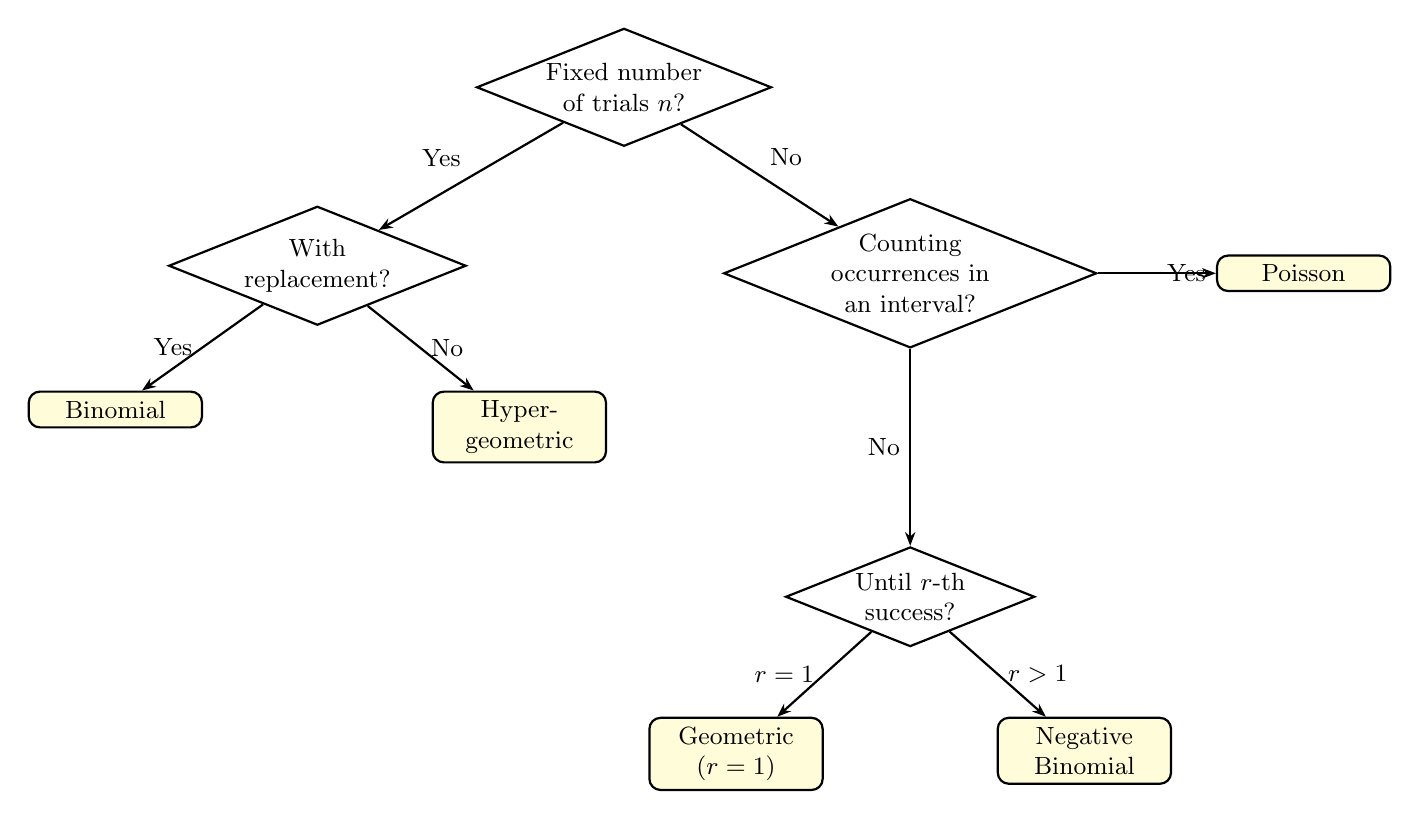
\begin{tikzpicture}[
  node distance=1.2cm and 2.5cm,
  every node/.style={font=\small},
  decision/.style={draw, diamond, aspect=2.5, inner sep=1pt, align=center, thick},
  result/.style={draw, rounded corners, thick, fill=yellow!15, align=center, minimum width=2.2cm},
  arr/.style={-{Stealth[length=5pt]}, thick},
]
  \node[decision] (n) {Fixed number\\of trials $n$?};
  \node[decision, below left=1.5cm and 2cm of n] (replace) {With\\replacement?};
  \node[decision, below right=1.5cm and 1.5cm of n] (count) {Counting\\occurrences in\\an interval?};

  \node[result, below left=1.2cm and 0.5cm of replace] (bin) {Binomial};
  \node[result, below right=1.2cm and 0.5cm of replace] (hg) {Hyper-\\geometric};

  \node[decision, below=2.5cm of count] (rsuccess) {Until $r$-th\\success?};
  \node[result, right=1.5cm of count] (pois) {Poisson};
  \node[result, below left=1.2cm and 0.3cm of rsuccess] (geo) {Geometric\\($r=1$)};
  \node[result, below right=1.2cm and 0.3cm of rsuccess] (nb) {Negative\\Binomial};

  \draw[arr] (n) -- node[above left] {Yes} (replace);
  \draw[arr] (n) -- node[above right] {No} (count);
  \draw[arr] (replace) -- node[left] {Yes} (bin);
  \draw[arr] (replace) -- node[right] {No} (hg);
  \draw[arr] (count) -- node[right] {Yes} (pois);
  \draw[arr] (count) -- node[left] {No} (rsuccess);
  \draw[arr] (rsuccess) -- node[left] {$r=1$} (geo);
  \draw[arr] (rsuccess) -- node[right] {$r>1$} (nb);
\end{tikzpicture}
\end{center}

\end{secbody}

% ==========================================================
\section{Distribution Summary Table}
\label{sec:ov-table}
% ==========================================================

\begin{secbody}

\begin{center}
\renewcommand{\arraystretch}{1.8}
\begin{tabular}{@{}lcccc@{}}
\toprule
\textbf{Distribution} & \textbf{PMF} $f(x)$ & \textbf{Support} & $\boldsymbol{\mu}$ & $\boldsymbol{\sigma^2}$ \\
\midrule
Uniform$(k)$
  & $\dfrac{1}{k}$
  & $1, 2, \ldots, k$
  & $\dfrac{k+1}{2}$
  & $\dfrac{k^2 - 1}{12}$ \\[4pt]
Ber$(p)$
  & $p^x (1-p)^{1-x}$
  & $0, 1$
  & $p$
  & $pq$ \\[4pt]
Bin$(n,p)$
  & $\dbinom{n}{x} p^x q^{n-x}$
  & $0, 1, \ldots, n$
  & $np$
  & $npq$ \\[4pt]
HG$(N, N_1, n)$
  & $\dfrac{\binom{N_1}{x}\binom{N-N_1}{n-x}}{\binom{N}{n}}$
  & see below
  & $n\dfrac{N_1}{N}$
  & $n\dfrac{N_1}{N}\dfrac{N-N_1}{N}\dfrac{N-n}{N-1}$ \\[4pt]
Geometric$(p)$
  & $q^{x-1} p$
  & $1, 2, 3, \ldots$
  & $\dfrac{1}{p}$
  & $\dfrac{q}{p^2}$ \\[4pt]
NB$(r, p)$
  & $\dbinom{x-1}{r-1} p^r q^{x-r}$
  & $r, r+1, \ldots$
  & $\dfrac{r}{p}$
  & $\dfrac{rq}{p^2}$ \\[4pt]
Poisson$(\lambda)$
  & $\dfrac{\lambda^x}{x!} e^{-\lambda}$
  & $0, 1, 2, \ldots$
  & $\lambda$
  & $\lambda$ \\
\bottomrule
\end{tabular}
\end{center}
where $q = 1 - p$. For HG, support is $\max\{0, n-(N-N_1)\} \le x \le \min\{n, N_1\}$.

\end{secbody}

% ==========================================================
\section{MGF Summary}
\label{sec:ov-mgf}
% ==========================================================

\begin{secbody}

The \textbf{Moment Generating Function} is $M_X(t) = \E(e^{tX})$.
Key property: $M_X^{(r)}(0) = \E(X^r)$.

\begin{center}
\renewcommand{\arraystretch}{1.6}
\begin{tabular}{@{}lc@{}}
\toprule
\textbf{Distribution} & $\boldsymbol{M_X(t)}$ \\
\midrule
$\text{Bin}(n, p)$       & $(pe^t + q)^n$ \\
$\text{Geometric}(p)$    & $\dfrac{pe^t}{1 - qe^t}, \; t < -\ln q$ \\
$\text{NB}(r, p)$        & $\left(\dfrac{pe^t}{1 - qe^t}\right)^r, \; t < -\ln q$ \\
$\text{Poisson}(\lambda)$ & $e^{\lambda(e^t - 1)}$ \\
\bottomrule
\end{tabular}
\end{center}

\end{secbody}

% ==========================================================
\section{Approximations and Inequalities}
\label{sec:ov-approx}
% ==========================================================

\begin{secbody}

\textbf{Binomial approximation of Hypergeometric:}
When $n/N \le 0.05$,
\[
  X \sim \text{HG}(N, N_1, n) \;\approx\; \text{Bin}(n, p = N_1/N).
\]

\textbf{Poisson approximation of Binomial:}
When $n$ is large and $p$ is small ($\lambda = np$ moderate),
\[
  X \sim \text{Bin}(n, p) \;\approx\; \text{Poisson}(\lambda = np).
\]

\textbf{Tchebycheff's Inequality:} For any distribution, $k > 1$,
\[
  \boxed{P(\mu - k\sigma \le X \le \mu + k\sigma) \ge 1 - \frac{1}{k^2}.}
\]

\end{secbody}


%%%%%%%%%%%%%%%%%%%%%%%%%%%%%%%%%%%%%%%%%%%%%%%%%%%%%%%%%%%%%
%%%%%%%%%%%%%%%%%%%%%%%%%%%%%%%%%%%%%%%%%%%%%%%%%%%%%%%%%%%%%
\newpage
\part{Detailed Notes --- Definitions, Proofs, and Examples}
\label{part:detailed}
%%%%%%%%%%%%%%%%%%%%%%%%%%%%%%%%%%%%%%%%%%%%%%%%%%%%%%%%%%%%%
%%%%%%%%%%%%%%%%%%%%%%%%%%%%%%%%%%%%%%%%%%%%%%%%%%%%%%%%%%%%%

% ==========================================================
\section{Random Variables}
\label{sec:det-rv}
% ==========================================================

\subsection{Definition and Classification}
\begin{sub}

\begin{definition}[Random Variable]
  A \textbf{random variable} (r.v.) $X$ is a rule or function that assigns a
  real number to each element $w$ in the sample space $S$ of a random
  experiment:
  \[
    X_{(w)} = x, \quad w \in S, \; x \in \R.
  \]
\end{definition}

\begin{definition}[Discrete Random Variable]
  A random variable is \textbf{discrete} if its set of possible values is
  finite or countably infinite.
\end{definition}

\begin{example}
  Toss a fair coin twice. Let $X = \#$ of heads.
  \begin{itemize}
    \item $S = \{HH, HT, TH, TT\}$.
    \item Possible values of $X$: $\{0, 1, 2\}$ --- finite, so $X$ is discrete.
  \end{itemize}
\end{example}

\begin{example}
  Toss a fair coin repeatedly until the first heads. Let $X = \#$ of tosses needed.
  \begin{itemize}
    \item Possible values: $\{1, 2, 3, \ldots\}$ --- countably infinite, so $X$ is discrete.
  \end{itemize}
\end{example}

\end{sub}

\subsection{Probability Mass Function}
\begin{sub}

\begin{definition}[PMF]
  \label{def:pmf}
  The \textbf{probability mass function} (p.m.f.) of a discrete random
  variable $X$ is
  \begin{equation}
    f(x) = P(X = x), \quad \text{for all } x \text{ such that } f(x) > 0.
    \label{eq:pmf}
  \end{equation}
\end{definition}

\begin{theorem}[Properties of a PMF]
  \label{thm:pmf-prop}
  \begin{enumerate}
    \item $0 \le f(x) \le 1$ for any $x$.
    \item $\displaystyle\sum_{\text{all } x} f(x) = 1$. \quad (Total probability)
    \item $\displaystyle P(a < X \le b) = \sum_{a < x \le b} f(x)$. \quad (Summation of PMF gives probability)
  \end{enumerate}
\end{theorem}

\begin{example}[PMF of coin toss]
  \label{ex:pmf-coin}
  Let $X = \#$ of heads from two tosses of a fair coin. Then $S = \{HH, HT, TH, TT\}$, and
  \begin{center}
    \begin{tabular}{c|ccc}
      $x$ & 0 & 1 & 2 \\ \hline
      $P(X = x)$ & $1/4$ & $1/2$ & $1/4$
    \end{tabular}
  \end{center}
  Verification: $\frac{1}{4} + \frac{1}{2} + \frac{1}{4} = 1$. \checkmark

  The probability of getting at least one heads:
  \[
    P(X \ge 1) = f(1) + f(2) = \tfrac{1}{2} + \tfrac{1}{4} = \tfrac{3}{4}.
  \]
\end{example}

\begin{example}[Finding a normalizing constant]
  \label{ex:find-c}
  Suppose $f(x) = cx$, $x = 1, 2, \ldots, 10$. Find $c$.

  By total probability:
  \[
    \sum_{x=1}^{10} cx = c \cdot \frac{10 \cdot 11}{2} = 55c = 1
    \implies c = \frac{1}{55}.
  \]
\end{example}

\end{sub}

\subsection{Cumulative Distribution Function}
\begin{sub}

\begin{definition}[CDF]
  \label{def:cdf}
  The \textbf{cumulative distribution function} (CDF) of r.v.\ $X$ is
  \begin{equation}
    F(x) = P(X \le x), \quad x \in \R.
    \label{eq:cdf}
  \end{equation}
  Note: $x$ may not be a value $X$ takes.
  If $X$ is discrete,
  \begin{equation}
    F(x) = \sum_{k \le x} P(X = k).
    \label{eq:cdf-disc}
  \end{equation}
\end{definition}

\begin{example}[CDF from PMF]
  \label{ex:cdf-coin}
  For $X = \#$ of heads from two fair coin tosses (Example~\ref{ex:pmf-coin}):
  \[
    F(x) = P(X \le x) =
    \begin{cases}
      0,    & x < 0, \\
      1/4,  & 0 \le x < 1, \\
      3/4,  & 1 \le x < 2, \\
      1,    & x \ge 2.
    \end{cases}
  \]
\end{example}

\begin{proposition}[Properties of the CDF]
  \label{prop:cdf-prop}
  For discrete $X$:
  \begin{enumerate}
    \item $F(x)$ is a piecewise right-continuous step function.
    \item Number of steps $=$ number of possible values of $X$.
    \item Amount of jump of $F(x)$ at $x$ is $f(x) = P(X = x)$.
    \item $F(x)$ is non-decreasing.
    \item $F(x) \to 0$ as $x \to -\infty$.
    \item $F(x) \to 1$ as $x \to \infty$.
  \end{enumerate}
\end{proposition}

\begin{example}[PMF from CDF]
  \label{ex:pmf-from-cdf}
  Given
  \[
    F(x) = \begin{cases}
      0,      & x < 0, \\
      10/13,  & 0 \le x < 1, \\
      1,      & x \ge 1.
    \end{cases}
  \]
  The jumps give the PMF: $f(0) = 10/13$ and $f(1) = 3/13$.

  This is the distribution of $X = \begin{cases} 1, & \text{if face card} \\ 0, & \text{if not} \end{cases}$ when selecting a card at random from a standard deck (12 face cards out of 52, so $P(X=1) = 12/52 = 3/13$).
\end{example}

\end{sub}

% ==========================================================
\section{Expected Value and Variance}
\label{sec:det-ev}
% ==========================================================

\subsection{Expected Value}
\begin{sub}

\begin{definition}[Expected Value]
  \label{def:ev}
  The \textbf{expected value} (mean) of a discrete r.v.\ $X$ is
  \begin{equation}
    \mu = \mu_X = \E(X) = \sum_{\text{all } x} x \, f(x).
    \label{eq:ev}
  \end{equation}
\end{definition}

\textbf{Two interpretations of $\mu$:}
\begin{enumerate}
  \item \textbf{Long-run average}: the average outcome if you repeat the experiment many times.
  \item \textbf{Balance point}: the center of gravity of the probability distribution.
\end{enumerate}

\begin{example}[Mean of a fair die]
  \label{ex:mean-die}
  Roll a fair six-sided die (Die \#1). Let $X =$ number on top.
  \[
    f(x) = \frac{1}{6}, \quad x = 1, 2, \ldots, 6.
  \]
  \[
    \mu = \sum_{x=1}^{6} x \cdot \frac{1}{6}
        = \frac{1}{6}(1 + 2 + 3 + 4 + 5 + 6)
        = \frac{21}{6} = 3.5.
  \]
\end{example}

\begin{example}[Die \#2 --- using a function of $X$]
  \label{ex:die2}
  Roll a die labeled $2, 4, 8, 16, 32, 64$ (Die \#2). Let $Y =$ number on top.
  Using Die~\#1 with $X =$ face number, we have $Y = 2^X$.
  \[
    \E(Y) = \E(2^X) = \sum_{x=1}^{6} 2^x \cdot \frac{1}{6}
           = \frac{1}{6}(2 + 4 + 8 + 16 + 32 + 64)
           = \frac{126}{6} = 21.
  \]
\end{example}

\end{sub}

\subsection{Expected Value of a Function of $X$}
\begin{sub}

\begin{theorem}[Law of the Unconscious Statistician]
  \label{thm:lotus}
  If $u(X)$ is a function of discrete r.v.\ $X$, then
  \begin{equation}
    \E\bigl(u(X)\bigr) = \sum_{\text{all } x} u(x) \, f(x).
    \label{eq:lotus}
  \end{equation}
\end{theorem}

\begin{remark}
  When $u(X) = X$, this reduces to $\E(X) = \sum x \, f(x)$.
\end{remark}

\begin{example}
  \label{ex:lotus}
  Let $X$ be a r.v.\ with PMF $f(x) = \frac{x}{10}$, $x = 1, 2, 3, 4$.
  \begin{enumerate}
    \item Find $\E(Y)$ where $Y = X^2$.
      \begin{align*}
        \E(X^2) &= \sum_{x=1}^{4} x^2 \cdot \frac{x}{10}
                 = \frac{1}{10}(1 + 8 + 27 + 64) = \frac{100}{10} = 10.
      \end{align*}
    \item Find $\E(1/X^2)$.
      \begin{align*}
        \E\!\left(\frac{1}{X^2}\right)
          &= \sum_{x=1}^{4} \frac{1}{x^2} \cdot \frac{x}{10}
           = \frac{1}{10}\!\left(1 + \frac{1}{2} + \frac{1}{3} + \frac{1}{4}\right)
           = \frac{1}{10} \cdot \frac{25}{12}
           = \frac{25}{120} = \frac{5}{24}.
      \end{align*}
  \end{enumerate}
\end{example}

\end{sub}

\subsection{Linearity of Expectation}
\begin{sub}

\begin{theorem}[Linearity of $\E$]
  \label{thm:linearity}
  \leavevmode
  \begin{enumerate}
    \item $\E(c) = c$ for any constant $c$.
    \item $\E\bigl(c \, u(X)\bigr) = c \, \E\bigl(u(X)\bigr)$.
    \item $\E\bigl(c_1 u_1(X) + c_2 u_2(X)\bigr) = c_1 \E\bigl(u_1(X)\bigr) + c_2 \E\bigl(u_2(X)\bigr)$.
  \end{enumerate}
  More generally,
  \begin{equation}
    \E\Bigl(c_0 + \sum_{i=1}^{n} c_i u_i(X)\Bigr) = c_0 + \sum_{i=1}^{n} c_i \, \E\bigl(u_i(X)\bigr).
    \label{eq:linearity}
  \end{equation}
  That is, $\E$ is a \textbf{linear operator}:
  \begin{itemize}
    \item The expected value of a sum is the sum of the expected values.
    \item The expected value of a constant times a function is the constant times the expected value.
  \end{itemize}
\end{theorem}

\begin{example}
  \label{ex:linearity}
  Suppose $\E(X) = 3$ and $\E(X^2) = 10$. Find $\E\bigl((X-5)^2\bigr)$.
  \begin{align*}
    \E\bigl((X-5)^2\bigr)
      &= \E(X^2 - 10X + 25) \\
      &= \E(X^2) - 10\E(X) + 25 \\
      &= 10 - 30 + 25 = 5.
  \end{align*}
\end{example}

\begin{example}[Fair game]
  \label{ex:fair-game}
  One pays \$20 to roll Die \#2 (labeled $2, 4, 8, 16, 32, 64$) and receives a cash reward equal to the number on top.

  Gain $= Y - 20$ where $Y$ is the face value. Since $\E(Y) = 21$ (Example~\ref{ex:die2}),
  \[
    \E(\text{Gain}) = \E(Y) - 20 = 21 - 20 = 1 > 0.
  \]
  The game is \emph{not} fair --- it slightly favors the player.
\end{example}

\end{sub}

\subsection{Variance and Standard Deviation}
\begin{sub}

\begin{definition}[Variance]
  \label{def:var}
  The \textbf{variance} of r.v.\ $X$ is the weighted average squared distance
  between $X$ and its mean:
  \begin{equation}
    \sigma^2 = \Var(X) = \E\bigl((X - \mu)^2\bigr).
    \label{eq:var-def}
  \end{equation}
  For discrete $X$:
  \begin{equation}
    \sigma^2 = \sum_{\text{all } x} (x - \mu)^2 f(x).
    \label{eq:var-disc}
  \end{equation}
\end{definition}

\begin{theorem}[Shortcut formula for variance]
  \label{thm:var-shortcut}
  For any random variable $X$,
  \begin{equation}
    \boxed{\sigma^2 = \E(X^2) - \mu^2.}
    \label{eq:var-shortcut}
  \end{equation}
\end{theorem}

\begin{proof}
  Expand the definition:
  \begin{align*}
    \sigma^2
      &= \E\bigl((X - \mu)^2\bigr) \\
      &= \E(X^2 - 2\mu X + \mu^2) \\
      &= \E(X^2) - 2\mu \, \E(X) + \mu^2 \\
      &= \E(X^2) - 2\mu^2 + \mu^2 \\
      &= \E(X^2) - \mu^2. \qedhere
  \end{align*}
\end{proof}

\begin{remark}
  Why not use $\E(X - \mu)$ as a measure of spread?
  Because $\E(X - \mu) = \E(X) - \mu = \mu - \mu = 0$ always.
  Squaring prevents cancellation of positive and negative deviations.
\end{remark}

\begin{definition}[Standard Deviation]
  \label{def:sd}
  \begin{equation}
    \sigma = \SD(X) = \sqrt{\sigma^2}.
    \label{eq:sd}
  \end{equation}
  The standard deviation has the \textbf{same unit} as $X$.
\end{definition}

\end{sub}

\subsection{Mean and Variance of $a + bX$}
\begin{sub}

\begin{theorem}
  \label{thm:linear-transform}
  For constants $a, b$ and random variable $X$:
  \begin{align}
    \E(a + bX) &= a + b\,\mu, \label{eq:linear-mean} \\
    \Var(a + bX) &= b^2 \sigma^2. \label{eq:linear-var}
  \end{align}
\end{theorem}

\begin{proof}
  Mean: $\E(a + bX) = a + b\,\E(X) = a + b\mu$ by linearity.

  Variance: Let $Y = a + bX$. Then $\mu_Y = a + b\mu$, so
  \begin{align*}
    \Var(Y) &= \E\bigl((Y - \mu_Y)^2\bigr) = \E\bigl((bX + a - a - b\mu)^2\bigr) \\
            &= \E\bigl(b^2(X - \mu)^2\bigr) = b^2 \E\bigl((X-\mu)^2\bigr) = b^2 \sigma^2. \qedhere
  \end{align*}
\end{proof}

\begin{example}
  If $\Var(5X - 1) = 9$, find $\sigma_X^2$.

  $\Var(5X - 1) = 5^2 \sigma_X^2 = 25\sigma_X^2 = 9$, so $\sigma_X^2 = 9/25$.
\end{example}

\begin{example}
  Suppose $\E\bigl((5X-1)^2\bigr) = 10$ and $\E(5X - 1) = 1$. Find $\E(X)$ and $\Var(5X-1)$.

  From $\E(5X - 1) = 5\E(X) - 1 = 1$, we get $\E(X) = 2/5$.

  $\Var(5X - 1) = \E\bigl((5X-1)^2\bigr) - \bigl(\E(5X-1)\bigr)^2 = 10 - 1 = 9$.
\end{example}

\end{sub}

% ==========================================================
\section{Discrete Uniform Distribution}
\label{sec:det-uniform}
% ==========================================================

\subsection{Definition and Properties}
\begin{sub}

\begin{definition}[Discrete Uniform]
  Random variable $X$ has a \textbf{Discrete Uniform Distribution} if it
  takes values $1, 2, \ldots, k$ with equal probability.
  Denote $X \sim \text{Uniform}(k)$.
\end{definition}

\textbf{PMF:}
\begin{equation}
  f(x) = P(X = x) = \frac{1}{k}, \quad x = 1, 2, \ldots, k.
  \label{eq:uniform-pmf}
\end{equation}

\textbf{CDF:}
\[
  F(x) = P(X \le x) = \sum_{t \le x} P(X = t).
\]

\textbf{Mean and Variance:}
\begin{equation}
  \mu = \frac{k + 1}{2}, \qquad
  \sigma^2 = \frac{k^2 - 1}{12}.
  \label{eq:uniform-params}
\end{equation}

\begin{example}[Fair die]
  Roll a fair six-sided die: $X \sim \text{Uniform}(6)$.
  \begin{enumerate}
    \item[(a)] $f(x) = 1/6$ for $x = 1, \ldots, 6$.
    \item[(b)] $P(X \ge 5) = f(5) + f(6) = 2/6 = 1/3$.
    \item[(c)] $\mu = 7/2 = 3.5$, \; $\sigma^2 = 35/12 \approx 2.917$.
  \end{enumerate}
\end{example}

\end{sub}

% ==========================================================
\section{Hypergeometric Distribution}
\label{sec:det-hg}
% ==========================================================

\subsection{Definition}
\begin{sub}

\begin{definition}[Hypergeometric]
  A finite population of size $N$ consists of two types: $N_1$ of type~I
  and $N - N_1$ of type~II. A sample of size $n$ is taken \textbf{without
  replacement}. Let $X$ = number of type~I members in the sample.
  Then $X \sim \text{HG}(N, N_1, n)$.
\end{definition}

\textbf{PMF:}
\begin{equation}
  f(x) = P(X = x) = \frac{\binom{N_1}{x}\binom{N - N_1}{n - x}}{\binom{N}{n}},
  \quad \max\{0, n - (N - N_1)\} \le x \le \min\{n, N_1\}.
  \label{eq:hg-pmf}
\end{equation}

\textbf{Mean and Variance:}
\begin{equation}
  \mu = n \cdot \frac{N_1}{N}, \qquad
  \sigma^2 = n \cdot \frac{N_1}{N} \cdot \frac{N - N_1}{N} \cdot \frac{N - n}{N - 1}.
  \label{eq:hg-params}
\end{equation}

\end{sub}

\subsection{Example}
\begin{sub}

\begin{example}[Tagged fish]
  \label{ex:fish}
  There are 9 fish in a pond, 3 of which are tagged. Randomly catch 7 fish.
  Let $X = \#$ of tagged fish caught.

  $X \sim \text{HG}(N=9, N_1=3, n=7)$.

  \begin{enumerate}
    \item[(a)] Support: $\max\{0, 7-6\} = 1 \le x \le \min\{7, 3\} = 3$.
    \item[(b)] $P(X \le 1) = P(X = 1) = \dfrac{\binom{3}{1}\binom{6}{6}}{\binom{9}{7}}
              = \dfrac{3 \cdot 1}{36} = \dfrac{1}{12}$.
    \item[(c)] $\mu = 7 \cdot \dfrac{3}{9} = \dfrac{7}{3} \approx 2.333$.

              $\sigma^2 = 7 \cdot \dfrac{3}{9} \cdot \dfrac{6}{9} \cdot \dfrac{2}{8} = \dfrac{7}{27} \approx 0.346$ (using $\frac{N-n}{N-1} = \frac{2}{8}$).
  \end{enumerate}
\end{example}

\end{sub}

% ==========================================================
\section{Bernoulli and Binomial Distributions}
\label{sec:det-binom}
% ==========================================================

\subsection{Bernoulli Trial and Indicator Random Variable}
\begin{sub}

\begin{definition}[Bernoulli Trial]
  A \textbf{Bernoulli trial} is a random experiment whose outcomes are
  dichotomized into ``success'' and ``failure.''
\end{definition}

\begin{definition}[Bernoulli Random Variable]
  An \textbf{indicator random variable} (Bernoulli r.v.) takes only values 0
  and 1 based on a Bernoulli trial.
  Let $p = P(X = 1) = P(\text{success})$. Denote $X \sim \text{Ber}(p)$.

  \textbf{PMF:}
  \begin{equation}
    f(x) = p^x (1-p)^{1-x}, \quad x = 0, 1.
    \label{eq:ber-pmf}
  \end{equation}

  \textbf{Mean:} $\mu = p$. \quad
  \textbf{Variance:} $\sigma^2 = p(1-p) = pq$. \quad
  \textbf{SD:} $\sigma = \sqrt{pq}$.
\end{definition}

\end{sub}

\subsection{Binomial Distribution}
\begin{sub}

\begin{definition}[Binomial Experiment]
  A \textbf{binomial experiment} is a sequence of independent and identical
  Bernoulli trials satisfying:
  \begin{enumerate}
    \item Fixed number $n$ of trials.
    \item Each trial has 2 outcomes: success and failure.
    \item $p = P(\text{success})$ is constant across trials; $q = 1 - p$.
    \item Trials are independent.
  \end{enumerate}
\end{definition}

\begin{definition}[Binomial Random Variable]
  Let $X =$ total number of successes in a binomial experiment. Then $X$
  is a \textbf{Binomial Random Variable}, denoted $X \sim \text{Bin}(n, p)$.
  Note: $\text{Bin}(1, p) \equiv \text{Ber}(p)$.
\end{definition}

\textbf{PMF:}
\begin{equation}
  f(x) = P(X = x) = \binom{n}{x} p^x q^{n-x}, \quad x = 0, 1, \ldots, n.
  \label{eq:binom-pmf}
\end{equation}

\textbf{Verification (total probability):}
\[
  \sum_{x=0}^{n} f(x) = \sum_{x=0}^{n} \binom{n}{x} p^x q^{n-x} = (p + q)^n = 1^n = 1. \checkmark
\]
(by the Binomial Theorem)

\textbf{CDF:}
\[
  F(x) = P(X \le x) = \sum_{k \le x} f(k). \quad \text{(Use Binomial tables or calculator)}
\]

\end{sub}

\subsection{Mean and Variance of Binomial}
\begin{sub}

\begin{theorem}
  \label{thm:binom-mean}
  If $X \sim \text{Bin}(n, p)$, then $\mu = np$ and $\sigma^2 = npq$.
\end{theorem}

\textbf{Intuitive proof (Bernoulli decomposition):}

The key idea is that a Binomial is just the \textbf{sum of $n$ independent
Bernoulli trials}. Let $X_i$ be the outcome of the $i$-th trial:
\[
  X_i = \begin{cases} 1 & \text{(success), with probability } p, \\ 0 & \text{(failure), with probability } q. \end{cases}
\]
Then $X = X_1 + X_2 + \cdots + X_n$.

\textbf{Mean:} Linearity of $\E$ lets us split the sum:
\[
  \E(X) = \E(X_1) + \E(X_2) + \cdots + \E(X_n)
        = \underbrace{p + p + \cdots + p}_{n \text{ times}} = np.
\]
Example: flip a coin ($p=0.5$) ten times. Expected heads $= 10 \times 0.5 = 5$.

\textbf{Variance:} Each $X_i$ is independent, so variances also add:
\[
  \Var(X) = \Var(X_1) + \Var(X_2) + \cdots + \Var(X_n).
\]
For a single Bernoulli, since $X_i^2 = X_i$ (because $0^2=0$ and $1^2=1$):
\[
  \Var(X_i) = \E(X_i^2) - [\E(X_i)]^2 = p - p^2 = p(1-p) = pq.
\]
Therefore:
\[
  \Var(X) = \underbrace{pq + pq + \cdots + pq}_{n \text{ times}} = npq.
\]

\begin{remark}
  In short: Binomial $=$ sum of $n$ Bernoullis, so mean and variance are
  each just $n$ times the Bernoulli value.
\end{remark}

\medskip
\textbf{Formal proof of $\mu = np$ (via PMF):}
\begin{proof}
  \begin{align*}
    \E(X) &= \sum_{x=0}^{n} x \binom{n}{x} p^x q^{n-x}
           = \sum_{x=1}^{n} x \cdot \frac{n!}{x!(n-x)!} p^x q^{n-x} \\
          &= \sum_{x=1}^{n} \frac{n!}{(x-1)!(n-x)!} p^x q^{n-x} \\
          &= np \sum_{x=1}^{n} \frac{(n-1)!}{(x-1)!(n-x)!} p^{x-1} q^{n-x}.
  \end{align*}
  Let $k = x - 1$, $m = n - 1$:
  \[
    \E(X) = np \sum_{k=0}^{m} \binom{m}{k} p^k q^{m-k} = np(p+q)^m = np. \qedhere
  \]
\end{proof}

(Formal proof of $\sigma^2 = npq$ via MGF is given in Section~\ref{sec:det-mgf}.)

\textbf{Standard Deviation:}
\begin{equation}
  \sigma = \sqrt{npq}.
  \label{eq:binom-sd}
\end{equation}

\end{sub}

\subsection{Binomial Examples}
\begin{sub}

\begin{example}[Coin toss]
  \label{ex:binom-coin}
  Toss a fair coin 3 times. Let $X = \#$ of heads. Then $X \sim \text{Bin}(3, 0.5)$.
  \begin{enumerate}
    \item $P(X = 2) = \binom{3}{2}(0.5)^2(0.5)^1 = 3 \cdot 0.125 = 0.375$.
    \item $\mu = 3 \cdot 0.5 = 1.5$, \; $\sigma^2 = 3 \cdot 0.5 \cdot 0.5 = 0.75$.
  \end{enumerate}
\end{example}

\begin{example}[Guessing on an exam]
  \label{ex:binom-exam}
  10 multiple-choice problems, 4 choices each, one correct. Bart guesses on all.
  Let $X = \#$ correct. Then $X \sim \text{Bin}(10, 0.25)$.
  \begin{enumerate}
    \item $P(X = 6) = \binom{10}{6}(0.25)^6(0.75)^4 \approx 0.0162$.
    \item $P(\text{passing}) = P(X \ge 6) = 1 - P(X \le 5) \approx 1 - 0.9803 = 0.0197$.
    \item $P(2 \le X < 5) = P(X \le 4) - P(X \le 1) \approx 0.9219 - 0.2440 = 0.6779$.
    \item Expected correct: $\mu = 10 \cdot 0.25 = 2.5$.
  \end{enumerate}
\end{example}

\end{sub}

\subsection{Tchebycheff's Inequality}
\begin{sub}

\begin{theorem}[Tchebycheff's Inequality]
  \label{thm:tchebycheff}
  For any distribution (discrete or continuous; symmetric or skewed),
  for $k > 1$:
  \begin{equation}
    \boxed{P(\mu - k\sigma \le X \le \mu + k\sigma) \ge 1 - \frac{1}{k^2}.}
    \label{eq:tchebycheff}
  \end{equation}
\end{theorem}

\begin{example}
  For Bart's exam ($X \sim \text{Bin}(10, 0.25)$), verify for $k = 2$:
  \begin{itemize}
    \item $\mu = 2.5$, $\sigma = \sqrt{10 \cdot 0.25 \cdot 0.75} = \sqrt{1.875} \approx 1.369$.
    \item Interval: $\mu \pm 2\sigma = (2.5 - 2.738, \; 2.5 + 2.738) = (-0.238, \; 5.238)$.
    \item $P(-0.238 \le X \le 5.238) = P(0 \le X \le 5) \approx 0.9803 \ge 0.75 = 1 - 1/4$. \checkmark
  \end{itemize}
\end{example}

\end{sub}

\subsection{Binomial Approximation of Hypergeometric}
\begin{sub}

When sampling \textbf{without replacement} from a large population, the
hypergeometric distribution is well-approximated by the binomial.

\begin{theorem}
  For $X \sim \text{HG}(N, N_1, n)$, when $\dfrac{n}{N} \le 0.05$,
  \[
    X \;\overset{\cdot}{\sim}\; \text{Bin}\!\left(n, \; p = \frac{N_1}{N}\right).
  \]
\end{theorem}

\begin{example}
  A group of 1000 people: 850 left-handed, 150 right-handed.
  Select 4 at random. Let $X = \#$ right-handed.

  Exact: $X \sim \text{HG}(1000, 150, 4)$.
  Since $n/N = 4/1000 = 0.004 \le 0.05$, approximate by $X \sim \text{Bin}(4, 0.15)$.
  \[
    P(X = 1) \approx \binom{4}{1}(0.15)^1(0.85)^3 \approx 0.3685.
  \]
  True value: $\dfrac{\binom{150}{1}\binom{850}{3}}{\binom{1000}{4}} \approx 0.3694$.
\end{example}

\end{sub}

% ==========================================================
\section{Moment Generating Function}
\label{sec:det-mgf}
% ==========================================================

\subsection{Moments}
\begin{sub}

\begin{definition}[Moments]
  $\E(X^r)$ is called the \textbf{$r$-th moment} of the distribution of $X$,
  for $r = 1, 2, \ldots$.
  \begin{itemize}
    \item $\mu = \E(X)$ is the 1st moment.
    \item $\E(X^2)$ is the 2nd moment.
    \item $\sigma^2 = \E(X^2) - [\E(X)]^2$ = 2nd moment $-$ (1st moment)$^2$.
  \end{itemize}
\end{definition}

\end{sub}

\subsection{Definition and Properties of MGF}
\begin{sub}

\begin{definition}[MGF]
  The \textbf{moment generating function} of r.v.\ $X$ is
  \begin{equation}
    \boxed{M_X(t) = \E(e^{tX}),}
    \label{eq:mgf-def}
  \end{equation}
  provided $\E(e^{tX}) < \infty$ for $t$ in an interval containing 0.

  If $X$ is discrete: $M_X(t) = \sum_{\text{all } x} e^{tx} f(x)$.
\end{definition}

\textbf{Key properties:}
\begin{itemize}
  \item $M_X(0) = \E(e^{0 \cdot X}) = \E(1) = 1$.
  \item $M_X(t)$ is a function of $t$ (not $x$).
  \item Like the PMF and CDF, $M_X(t)$ uniquely determines a distribution.
  \item \textbf{MGF produces moments:}
\end{itemize}

\begin{theorem}[MGF and Moments]
  \label{thm:mgf-moments}
  \begin{equation}
    \boxed{M_X^{(r)}(0) = \E(X^r), \quad r = 1, 2, \ldots}
    \label{eq:mgf-moments}
  \end{equation}
  That is, the $r$-th derivative of $M_X(t)$ evaluated at $t = 0$ gives
  the $r$-th moment.
\end{theorem}

\begin{proof}[Proof sketch]
  $M_X(t) = \E(e^{tX}) = \sum e^{tx} f(x)$.

  Differentiating with respect to $t$:
  \[
    M_X'(t) = \sum x \, e^{tx} f(x).
  \]
  Setting $t = 0$: $M_X'(0) = \sum x \, f(x) = \E(X)$.

  Differentiating again:
  \[
    M_X''(t) = \sum x^2 e^{tx} f(x), \quad
    M_X''(0) = \sum x^2 f(x) = \E(X^2).
  \]

  In general, $M_X^{(r)}(0) = \E(X^r)$.
\end{proof}

\begin{example}[MGF of coin toss]
  \label{ex:mgf-coin}
  $X = \#$ heads from 2 fair coin tosses. PMF: $f(0) = 1/4$, $f(1) = 1/2$, $f(2) = 1/4$.
  \[
    M_X(t) = \frac{1}{4}e^{0} + \frac{1}{2}e^{t} + \frac{1}{4}e^{2t}
           = \frac{1}{4}(1 + 2e^t + e^{2t})
           = \frac{1}{4}(1 + e^t)^2
           = \left(\frac{1}{2}e^t + \frac{1}{2}\right)^2.
  \]
  This matches $\text{Bin}(2, 0.5)$: $(pe^t + q)^n = (0.5 e^t + 0.5)^2$.
\end{example}

\begin{example}[Identifying distribution from MGF]
  If $M_X(t) = 0.2 + 0.8 e^t$, what is the PMF?

  $M_X(t) = \sum e^{tx} f(x) = f(0) e^{0} + f(1) e^{t} = 0.2 + 0.8 e^t$.

  So $f(0) = 0.2$, $f(1) = 0.8$. This is $\text{Ber}(0.8)$.
\end{example}

\end{sub}

\subsection{Skewness and Kurtosis}
\begin{sub}

\begin{definition}[Skewness]
  The \textbf{skewness} is the 3rd moment of the standardized $X$:
  \[
    \text{skewness} = \E\!\left[\left(\frac{X - \mu}{\sigma}\right)^3\right].
  \]
  \begin{itemize}
    \item Symmetric distribution: skewness $= 0$.
    \item Left-skewed: skewness $< 0$.
    \item Right-skewed: skewness $> 0$.
  \end{itemize}
  For $X \sim \text{Bin}(n,p)$: $\text{skewness} = \dfrac{1 - 2p}{\sqrt{npq}}$.
\end{definition}

\begin{definition}[Kurtosis]
  The \textbf{kurtosis} is the 4th moment of the standardized $X$:
  \[
    \text{kurtosis} = \E\!\left[\left(\frac{X - \mu}{\sigma}\right)^4\right].
  \]
  It measures ``tailedness.'' Normal distribution has kurtosis $= 3$.
  \begin{itemize}
    \item Kurtosis $= 3$: same tails as Normal.
    \item Kurtosis $< 3$: thinner tails than Normal.
    \item Kurtosis $> 3$: fatter tails than Normal.
  \end{itemize}
  For $X \sim \text{Bin}(n,p)$: $\text{kurtosis} = \dfrac{1 - 6p(1-p)}{npq} + 3$.
\end{definition}

\end{sub}

\subsection{MGF of Binomial --- Deriving Variance}
\begin{sub}

\begin{theorem}
  If $X \sim \text{Bin}(n, p)$, then
  \begin{equation}
    M_X(t) = (pe^t + q)^n.
    \label{eq:binom-mgf}
  \end{equation}
\end{theorem}

\begin{proof}
  \[
    M_X(t) = \sum_{x=0}^{n} e^{tx} \binom{n}{x} p^x q^{n-x}
           = \sum_{x=0}^{n} \binom{n}{x} (pe^t)^x q^{n-x}
           = (pe^t + q)^n
  \]
  by the Binomial Theorem.
\end{proof}

\textbf{Deriving $\E(X)$ and $\Var(X)$ via MGF:}

$M_X'(t) = n(pe^t + q)^{n-1} \cdot pe^t$.
\[
  \E(X) = M_X'(0) = n(p + q)^{n-1} \cdot p = np.
\]

$M_X''(t) = n(n-1)(pe^t + q)^{n-2}(pe^t)^2 + n(pe^t + q)^{n-1}(pe^t)$.
\[
  \E(X^2) = M_X''(0) = n(n-1)p^2 + np.
\]

Therefore:
\[
  \sigma^2 = \E(X^2) - \mu^2 = n(n-1)p^2 + np - n^2 p^2 = np - np^2 = np(1-p) = npq. \qed
\]

\end{sub}

% ==========================================================
\section{Geometric and Negative Binomial Distributions}
\label{sec:det-geo}
% ==========================================================

\subsection{Geometric Distribution}
\begin{sub}

\begin{definition}[Geometric]
  Let $X$ be the number of independent and identical Bernoulli trials
  needed to get the \textbf{first success}. Then $X \sim \text{Geometric}(p)$,
  where $p = P(\text{success})$.
\end{definition}

\textbf{PMF:}
\begin{equation}
  f(x) = P(X = x) = q^{x-1} p, \quad x = 1, 2, 3, \ldots
  \label{eq:geo-pmf}
\end{equation}

\textbf{Verification (total probability):}
\[
  \sum_{x=1}^{\infty} q^{x-1} p = p \sum_{x=1}^{\infty} q^{x-1}
  = p \cdot \frac{1}{1-q} = \frac{p}{p} = 1. \checkmark
\]
(Geometric series $\sum_{k=0}^{\infty} q^k = \frac{1}{1-q}$ for $|q| < 1$.)

\textbf{CDF:}
\begin{equation}
  F(x) = P(X \le x) = 1 - P(X > x) = 1 - q^{\lfloor x \rfloor}, \quad x \ge 1.
  \label{eq:geo-cdf}
\end{equation}

\textbf{MGF:}
\begin{equation}
  M_X(t) = \frac{pe^t}{1 - qe^t}, \quad t < -\ln q.
  \label{eq:geo-mgf}
\end{equation}

\textbf{Mean, Variance, SD:}
\begin{equation}
  \mu = \frac{1}{p}, \qquad \sigma^2 = \frac{q}{p^2}, \qquad \sigma = \frac{\sqrt{q}}{p}.
  \label{eq:geo-params}
\end{equation}

\begin{example}[Door-to-door sales]
  \label{ex:geo-cookies}
  One in twenty households makes a purchase ($p = 1/20 = 0.05$).
  Let $X = \#$ of households until the first sale. Then $X \sim \text{Geometric}(0.05)$.
  \begin{itemize}
    \item $P(\text{first sale at 5th household}) = (0.95)^4(0.05) \approx 0.0407$.
    \item $P(\text{first sale after 5th}) = P(X > 5) = q^5 = (0.95)^5 \approx 0.7738$.
  \end{itemize}
\end{example}

\begin{example}
  Roll a fair die repeatedly. Probability the first 5 occurs on the third roll:
  \[
    P(X = 3) = \left(\frac{5}{6}\right)^2 \cdot \frac{1}{6} = \frac{25}{216} \approx 0.1157.
  \]
\end{example}

\end{sub}

\subsection{Negative Binomial Distribution}
\begin{sub}

\begin{definition}[Negative Binomial]
  Let $X$ be the number of independent and identical Bernoulli trials needed
  to get $r$ \textbf{successes}. Then $X \sim \text{NB}(r, p)$.
\end{definition}

Note: $\text{NB}(1, p) \equiv \text{Geometric}(p)$.

\textbf{PMF:}
\begin{equation}
  f(x) = P(X = x) = \binom{x-1}{r-1} p^r q^{x-r}, \quad x = r, r+1, r+2, \ldots
  \label{eq:nb-pmf}
\end{equation}

\textbf{Interpretation:} The last trial (trial $x$) must be a success. Among the
first $x - 1$ trials, exactly $r - 1$ are successes: $\binom{x-1}{r-1} p^{r-1} q^{x-r}$.
Multiply by $p$ for the final success.

\textbf{Verification (total probability):}
Uses the Taylor series $(1 - y)^{-r} = \sum_{x=r}^{\infty} \binom{x-1}{r-1} y^{x-r}$.
\[
  \sum_{x=r}^{\infty} \binom{x-1}{r-1} p^r q^{x-r} = p^r (1-q)^{-r} = p^r \cdot p^{-r} = 1. \checkmark
\]

\textbf{MGF:}
\begin{equation}
  M_X(t) = \left(\frac{pe^t}{1 - qe^t}\right)^r, \quad t < -\ln q.
  \label{eq:nb-mgf}
\end{equation}

\textbf{Mean, Variance, SD} (derived via MGF):
\begin{equation}
  \mu = \frac{r}{p}, \qquad \sigma^2 = \frac{rq}{p^2}, \qquad \sigma = \frac{\sqrt{rq}}{p}.
  \label{eq:nb-params}
\end{equation}

\begin{proof}[Proof of mean and variance via MGF]
  Let $M(t) = \left(\frac{pe^t}{1 - qe^t}\right)^r$. Using the quotient rule:
  \[
    M'(t) = r\left(\frac{pe^t}{1 - qe^t}\right)^{r-1} \cdot \frac{pe^t(1-qe^t) + pe^t \cdot qe^t}{(1-qe^t)^2}
           = r\left(\frac{pe^t}{1-qe^t}\right)^{r-1} \cdot \frac{pe^t}{(1-qe^t)^2}.
  \]
  At $t = 0$: $M'(0) = r \cdot 1^{r-1} \cdot \frac{p}{p^2} = \frac{r}{p}$. So $\mu = r/p$.

  Similarly, $M''(0) = \frac{r^2 + rq}{p^2}$, giving
  \[
    \sigma^2 = \E(X^2) - \mu^2 = \frac{r^2 + rq}{p^2} - \frac{r^2}{p^2} = \frac{rq}{p^2}. \qedhere
  \]
\end{proof}

\begin{example}[Basketball free throws]
  \label{ex:nb-basketball}
  Practicing free throws, let $X = \#$ attempts to make $r = 10$ shots,
  with $p = P(\text{making a shot})$.
  Then $X \sim \text{NB}(10, p)$.

  $\E(X) = 10/p$. If $p = 0.8$, then on average $10/0.8 = 12.5$ attempts needed.
\end{example}

\begin{example}[Rolling dice]
  Roll a fair die repeatedly. Probability that at least 4 rolls are needed for the 3rd five:

  $X \sim \text{NB}(r=3, p=1/6)$. Want $P(X \ge 4) = 1 - P(X = 3)$.
  \[
    P(X = 3) = \binom{2}{2}\left(\frac{1}{6}\right)^3 \left(\frac{5}{6}\right)^0 = \frac{1}{216}.
  \]
  \[
    P(X \ge 4) = 1 - \frac{1}{216} = \frac{215}{216} \approx 0.9954.
  \]
\end{example}

\begin{example}[Identifying from MGF]
  If $M_X(t) = \left(\frac{0.75 e^t}{1 - 0.25 e^t}\right)^5$ for $t < -\ln 0.25$,
  identify the distribution.

  Comparing with~\eqref{eq:nb-mgf}: $p = 0.75$, $q = 0.25$, $r = 5$.
  So $X \sim \text{NB}(5, 0.75)$.

  $\mu = 5/0.75 = 20/3 \approx 6.67$, \;
  $\sigma^2 = 5 \cdot 0.25 / 0.75^2 = 20/9 \approx 2.22$.
\end{example}

\end{sub}

% ==========================================================
\section{Poisson Distribution}
\label{sec:det-poisson}
% ==========================================================

\subsection{Setting and Assumptions}
\begin{sub}

The Poisson distribution models $X = \#$ of occurrences of an event in a
fixed interval (1-D, 2-D, or 3-D).

\textbf{Assumptions:}
\begin{enumerate}
  \item Events happen one at a time.
  \item Rate of occurrence is constant over the entire interval.
  \item Events in non-overlapping intervals are independent. \quad (Memoryless property)
\end{enumerate}

Let $\lambda =$ average number of events in the interval (rate).
Then $X \sim \text{Poisson}(\lambda)$, with $x = 0, 1, 2, \ldots$

\end{sub}

\subsection{Derivation as Limit of Binomial}
\begin{sub}

Divide the interval into $n$ equal pieces. For large $n$, each piece
either has an event (probability $\lambda/n$) or not (by assumption~1).
So $X \sim \text{Bin}(n, \lambda/n)$ approximately.

As $n \to \infty$, $p = \lambda/n \to 0$, but $np = \lambda$ stays constant.

\begin{align*}
  P(X = x) &= \lim_{n \to \infty} \binom{n}{x} \left(\frac{\lambda}{n}\right)^x \left(1 - \frac{\lambda}{n}\right)^{n-x} \\
  &= \frac{\lambda^x}{x!} \lim_{n \to \infty} \frac{n(n-1)\cdots(n-x+1)}{n^x} \left(1 - \frac{\lambda}{n}\right)^n \left(1 - \frac{\lambda}{n}\right)^{-x} \\
  &= \frac{\lambda^x}{x!} \cdot 1 \cdot e^{-\lambda} \cdot 1
   = \frac{\lambda^x e^{-\lambda}}{x!}.
\end{align*}

\begin{remark}
  Poisson is the \textbf{limiting distribution} of Binomial as $n \to \infty$, $p \to 0$, with $np = \lambda$ fixed.
\end{remark}

\end{sub}

\subsection{PMF, MGF, and Parameters}
\begin{sub}

\textbf{PMF:}
\begin{equation}
  f(x) = P(X = x) = \frac{\lambda^x}{x!} e^{-\lambda}, \quad x = 0, 1, 2, \ldots
  \label{eq:pois-pmf}
\end{equation}

\textbf{Total probability:}
\[
  \sum_{x=0}^{\infty} \frac{\lambda^x}{x!} e^{-\lambda}
  = e^{-\lambda} \sum_{x=0}^{\infty} \frac{\lambda^x}{x!}
  = e^{-\lambda} \cdot e^{\lambda} = 1. \checkmark
\]
(Using Taylor series: $e^y = \sum_{x=0}^{\infty} \frac{y^x}{x!}$.)

\textbf{MGF:}
\begin{equation}
  M_X(t) = \sum_{x=0}^{\infty} e^{tx} \cdot \frac{\lambda^x}{x!} e^{-\lambda}
         = e^{-\lambda} \sum_{x=0}^{\infty} \frac{(e^t \lambda)^x}{x!}
         = e^{-\lambda} \cdot e^{\lambda e^t}
         = e^{\lambda(e^t - 1)}.
  \label{eq:pois-mgf}
\end{equation}

\textbf{Mean and Variance via MGF:}
\begin{align*}
  M_X'(t) &= e^{\lambda(e^t - 1)} \cdot \lambda e^t = M_X(t) \cdot \lambda e^t. \\
  \mu &= M_X'(0) = 1 \cdot \lambda = \lambda.
\end{align*}
\begin{align*}
  M_X''(t) &= \frac{\mathrm{d}}{\mathrm{d}t}\bigl(M_X(t) \cdot \lambda e^t\bigr)
            = M_X'(t) \cdot \lambda e^t + M_X(t) \cdot \lambda e^t. \\
  \E(X^2) &= M_X''(0) = \lambda \cdot \lambda + \lambda = \lambda^2 + \lambda.
\end{align*}
\[
  \sigma^2 = \E(X^2) - \mu^2 = \lambda^2 + \lambda - \lambda^2 = \lambda.
\]

\textbf{Summary:}
\begin{equation}
  \boxed{\mu = \lambda, \qquad \sigma^2 = \lambda, \qquad \sigma = \sqrt{\lambda}.}
  \label{eq:pois-params}
\end{equation}

\begin{remark}
  For a Poisson distribution, the mean and variance are \textbf{equal}.
  This is a useful diagnostic: if observed data has mean $\approx$ variance,
  Poisson may be a good model.
\end{remark}

\end{sub}

\subsection{Poisson Examples}
\begin{sub}

\begin{example}[Weekend accidents]
  \label{ex:pois-accidents}
  Number of accidents at an intersection on a given weekend has
  $X \sim \text{Poisson}(0.7)$.
  \begin{enumerate}
    \item[(a)] $P(X = 1) = \dfrac{0.7^1}{1!} e^{-0.7} = 0.7 e^{-0.7} \approx 0.3476$.
    \item[(b)] $P(X \ge 2) = 1 - P(X \le 1) = 1 - [P(X=0) + P(X=1)]$.

    $P(X=0) = e^{-0.7} \approx 0.4966$.

    $P(X \ge 2) = 1 - 0.4966 - 0.3476 \approx 0.1558$.
  \end{enumerate}
\end{example}

\begin{example}[Fabric defects]
  \label{ex:pois-fabric}
  A fabric has 3 defects per 1000 feet on average. Let $X = \#$ defects in
  a 1200-foot roll. The rate scales: $\lambda = 3 \cdot (1200/1000) = 3.6$.
  So $X \sim \text{Poisson}(3.6)$.
  \begin{enumerate}
    \item[(a)] $P(X = 0) = e^{-3.6} \approx 0.0273$.
    \item[(b)] $P(X < \mu - \sigma)$: $\mu = 3.6$, $\sigma = \sqrt{3.6} \approx 1.897$.

    $\mu - \sigma \approx 1.703$, so $P(X < 1.703) = P(X \le 1)$.

    $P(X \le 1) = P(X=0) + P(X=1) = e^{-3.6}(1 + 3.6) \approx 0.0273 + 0.0984 = 0.1257$.
  \end{enumerate}
\end{example}

\end{sub}

\subsection{Poisson Approximation of Binomial}
\begin{sub}

\textbf{Rule of thumb:} When $n$ is large and $p$ is small, with $\lambda = np$:
\[
  X \sim \text{Bin}(n, p) \;\approx\; \text{Poisson}(\lambda = np).
\]

\begin{example}[Defective light bulbs]
  A manufacturer produces $2\%$ defective bulbs. From a box of 100 bulbs,
  find $P(X \le 3)$ where $X = \#$ defective.

  Exact: $X \sim \text{Bin}(100, 0.02)$.
  $P(X \le 3) \approx 0.8590$.

  Approximate: $X \approx \text{Poisson}(\lambda = 100 \cdot 0.02 = 2)$.
  \[
    P(X \le 3) = \sum_{x=0}^{3} \frac{2^x}{x!} e^{-2}
               = e^{-2}\!\left(1 + 2 + 2 + \frac{4}{3}\right)
               \approx 0.8571.
  \]
  Good approximation. \checkmark
\end{example}

\end{sub}

% ==========================================================
\section{Roulette Wheel Games --- Variance Comparison}
\label{sec:det-roulette}
% ==========================================================

\begin{secbody}

A roulette wheel has 38 slots: 18 red, 18 black, 2 green.

\textbf{Game 1:} Bet \$1 on Black. Win \$1 if black, lose \$1 otherwise.

\textbf{Game 2:} Bet \$1 on a Number. Win \$35 if correct, lose \$1 otherwise.

Let $X =$ amount of money gained.

\begin{center}
\begin{tabular}{c|cc|c|cc}
\multicolumn{3}{c|}{\textbf{Game 1}} & \multicolumn{3}{c}{\textbf{Game 2}} \\
\hline
$x$ & 1 & $-1$ & $x$ & 35 & $-1$ \\
$f(x)$ & $18/38$ & $20/38$ & $f(x)$ & $1/38$ & $37/38$
\end{tabular}
\end{center}

Both games have the \textbf{same mean}:
\[
  \mu_1 = 1 \cdot \frac{18}{38} + (-1) \cdot \frac{20}{38} = -\frac{2}{38} = -\frac{1}{19} \approx -0.0526.
\]
\[
  \mu_2 = 35 \cdot \frac{1}{38} + (-1) \cdot \frac{37}{38} = -\frac{2}{38} = -\frac{1}{19} \approx -0.0526.
\]
Both games are NOT fair (expected loss of about 5.3 cents per dollar).

\textbf{But the variances differ greatly:}
\begin{align*}
  \sigma_1^2 &= \E(X_1^2) - \mu_1^2 = 1 \cdot 1 - (1/19)^2 = 1 - 1/361 \approx 0.9972. \\
  \sigma_2^2 &= 35^2 \cdot \frac{1}{38} + 1 \cdot \frac{37}{38} - (1/19)^2
             = \frac{1225 + 37}{38} - \frac{1}{361} \approx 33.208.
\end{align*}
\[
  \sigma_1 \approx 0.999, \qquad \sigma_2 \approx 5.763.
\]

Game~2 has much higher variance --- much more volatile, even though the
expected loss per bet is the same.

\end{secbody}

\end{document}
